\subsection{Overview}
As stated above, each subsystem has to accomplish its own goal. In particular, we can see AutomatedSOS and Track4Run as simple, three-tier applications, while Data4Help should display a more complex, scalability-oriented architecture.

The figure below gives a general overview of a possible implementation of the system.

\FloatBarrier

\begin{figure}[!h]
	\centering
	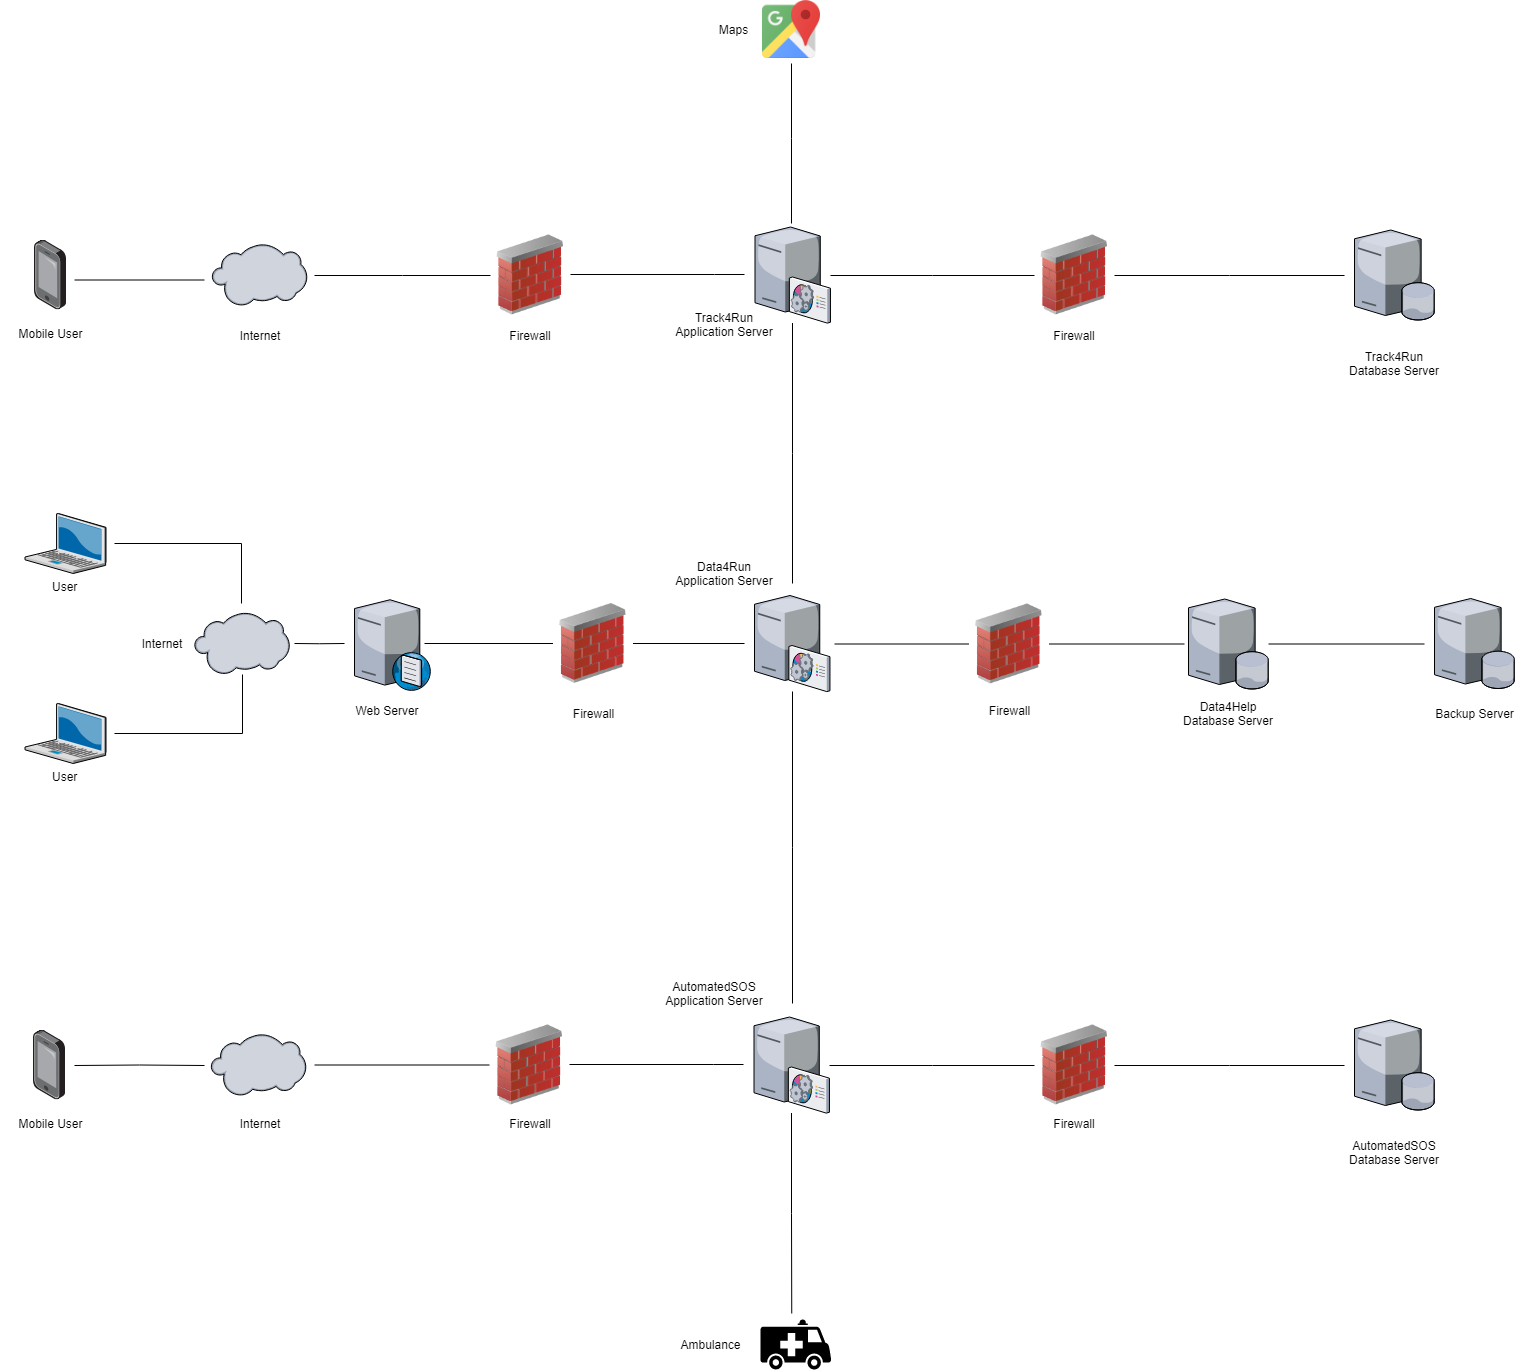
\includegraphics[width=\columnwidth]{physicalArchitectureDiagram.png}
	\caption{General Architecture}
\end{figure}


\FloatBarrier

As displayed in this figure, Data4Help subsystem's services can be accessed by many channels, including a web interface for users and APIs for data-sources and third-parties.
Since the data-sources provide real-time data from the user's devices, it is predictable that this flow of information will soon grow into a huge number of requests, so this subsystem has to be designed to quickly accomplish horizontal scaling and maintain high availability even in extreme conditions.
For this reason, a Microservice based architecture enforced with Message Queues and scalable databases should be adopted, as will be described in the following sections. Also an API Gateway is used to access all Data4Help interfaces, so to easily manage authentication and load balancing from the very first moment of any request.

AutomatedSOS and Track4Run instead are designed as applications with a thick client (i.e. smart-phone and smart-watch apps), a lightweight back-end server and a storage module. This design has been chosen because it is completely modular on one hand, since the two application's business logic is separated from Data4Help's one, but guarantees on the other hand a fast and reliable service provided by the servers, leaving the full responsibility of the presentation part to the mobile application. The separation of presentation and business logic also guarantees the maintainability of the system and good performances on mobile devices, where power consumption and CPU usage can be an issue.

\subsection{High Level Architecture}

From the component point of view, each subsystem can be divided into \textit{back-end} components, which are responsible of carrying out the business logic of the subsystem, and \textit{front-end} components, which provide a presentation layer to end users and SDKs to external developers who want to access the system's services.
Also, some external components are used to provide some of the services offered by the system.
In the following diagram, the main components and interfaces are highlighted, to give a general idea of the design of the system.
It must be noted that in this diagram components and \textit{modules} represent a set of services grouped together, and that internal interaction between modules is not shown for sake of simplicity: the complete description of all the modules and internal interfaces can be found in the following sections.

\FloatBarrier
\begin{figure}[!h]
	\centering
	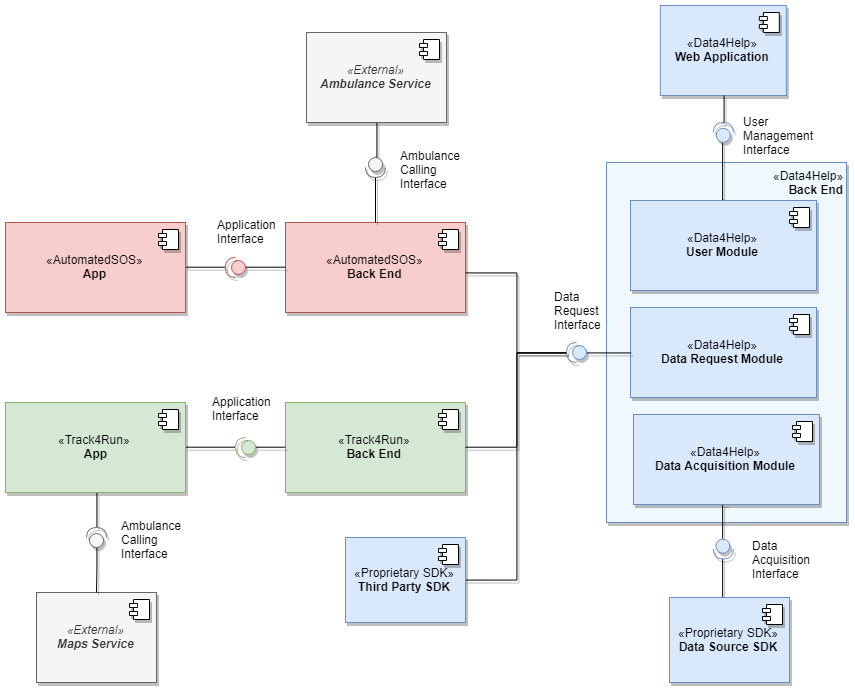
\includegraphics[width=\columnwidth]{ComponentDiagrams-Total.png}
	\caption{High Level Components}
\end{figure}
\FloatBarrier

As can be seen, the Data4Help back-end offers three main functionalities:

\begin{itemize}
	\item \textit{User Management}: provides an interface for managing the user account and configure his data-sources. This interface is exploited by a \textit{Web Application} that can be accessed via web browser.
	\item \textit{Data Acquisition}: provides the interface for collecting data from data-sources. A proprietary \textit{Data Source SDK} can be offered to external developers to integrate the use of this interface into their software and send data from external devices to Data4Help.
	\item \textit{User Management}: enables third parties to make requests on the data received by the subsystem. This interface is used by \textit{Track4Run} and \textit{AutomatedSOS} back-ends, but it can also be accessed by any other third party via the dedicated \textit{Third Party SDK}.
\end{itemize}

The other two back-ends are mainly responsible of exploiting Data4Help's serviced to offer an interface to the user's Application. 
For AutomatedSOS, an external ambulance calling interface is also needed by the back-end to fulfill its goal, while in Track4Run a Maps Service such as \textit{Google Maps} should be accessed directly from the Application to minimize latency and bandwidth occupation in the communication between the client and the server.

Another definition of the services offered by the system can be found in the figure below, which highlights the dependencies between the Data4Help system and its actors and provides a list of the services consumed internally and externally by the system.

\FloatBarrier
\begin{figure}[!h]
	\centering
	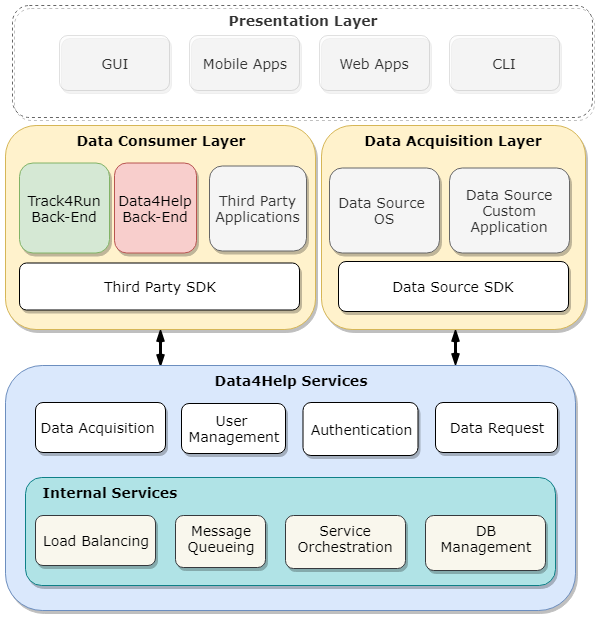
\includegraphics[width=0.8\columnwidth]{ComponentDiagrams-Layers.png}
	\caption{High Level Components}
\end{figure}
\FloatBarrier

\newpage
\subsection{Component View}


\subsubsection{Data4Help}

When considering the architecture for Data4Help, the first thing to take in account is scaling and availability. Data-sources can produce a lot of traffic, and vital services built on top of this subsystem, such as AutomatedSOS, bring the need for the system to handle all the data without losses, latency or service unavailability.
Bearing this in mind, the general idea of this subsystem's design is to exploit the new patterns of microservices and messages queues. 

The main focus of this design is that every service should be replicable in any desired number of instances (\textit{horizontal scaling}) without the need of changing other parts of the system. For this to be possible, the system must be provided with the following capabilities:

\begin{itemize}
	\item \textit{Container Environment}
	\item \textit{Container Orchestration}
	\item \textit{Load Balancing}
\end{itemize}

Future developments of the system can also add performance monitoring services, to test in real-time the stress level of the system and eventually deploy new instances of some services where needed.

This said, here is a detailed view of the components of this subsystem: each service is to be considered as independently deployed in a container, which is managed by the \textit{orchestrator}. For the sake of simplicity, only the interaction between developed components is highlighted, while the components dedicated to load balancing, orchestration and services deployment are considered to be already present as part of the \textit{API Gateway}.


\FloatBarrier
\begin{figure}[!h]
	\centering
	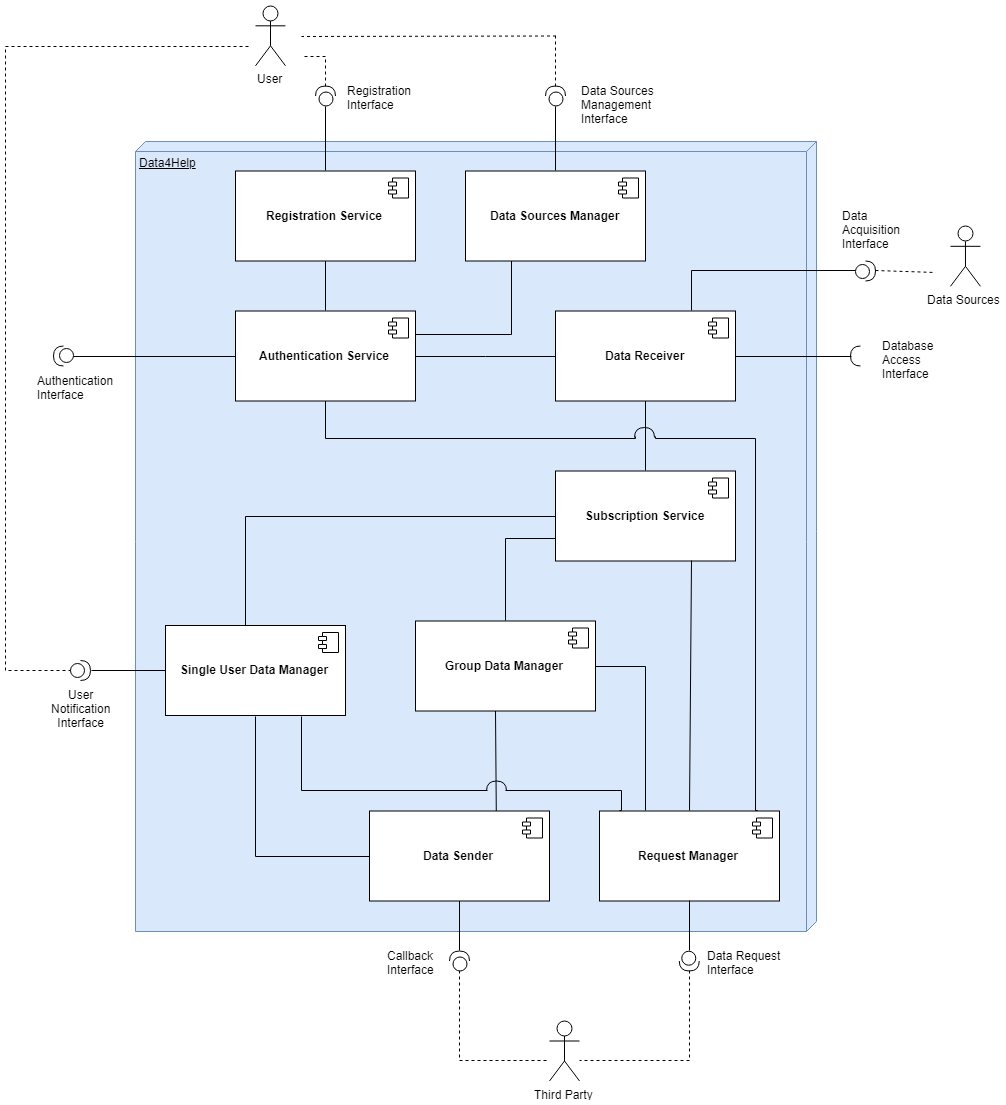
\includegraphics[width=\columnwidth]{ComponentDiagrams-Data4Help.png}
	\caption{Data4Help Components}
\end{figure}

\FloatBarrier

The internal microservices that have been identified are:
\begin{itemize}
	\item \textbf{Authentication Service}
	\item \textbf{User Service}
	\item \textbf{Receiver}
	\item \textbf{Request Manager}
	\item \textbf{Sender}
	\item \textbf{Subscription Service}
	\item \textbf{Anonymization Service}
\end{itemize}

This subsystem shall also use messaging between microservices where asyncronous communication is possible, in particular:

\begin{itemize}
	\item \textbf{New Data Queue}
	\item \textbf{New Request Queue}
	\item \textbf{Notification Queue}
	\item \textbf{Sending Queue}
\end{itemize}

All other components shall use synchronous protocols, such as RESTful APIs.

\subsubsection{AutomatedSOS}

\begin{figure}[!h]
	\centering
	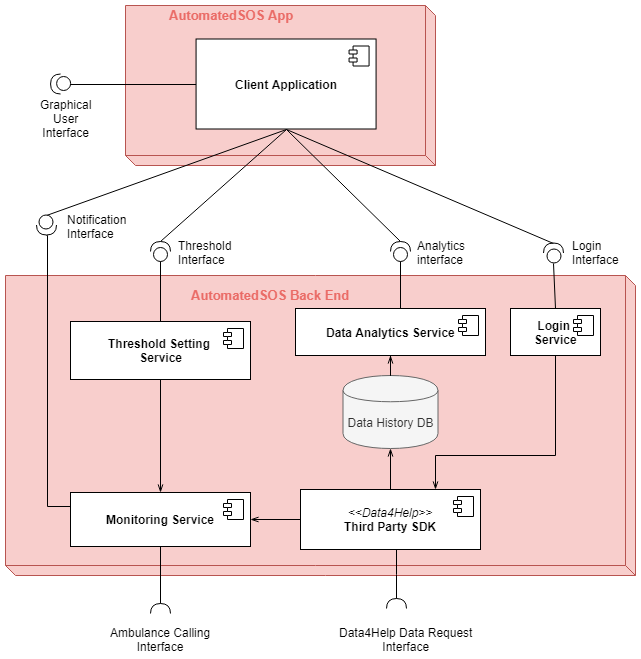
\includegraphics[width=\columnwidth]{ComponentDiagrams-AutoSOS.png}
	\caption{AutomatedSOS Components}
\end{figure}

\FloatBarrier


\subsubsection{Track4Run}

\FloatBarrier
\begin{figure}[!h]
	\centering
	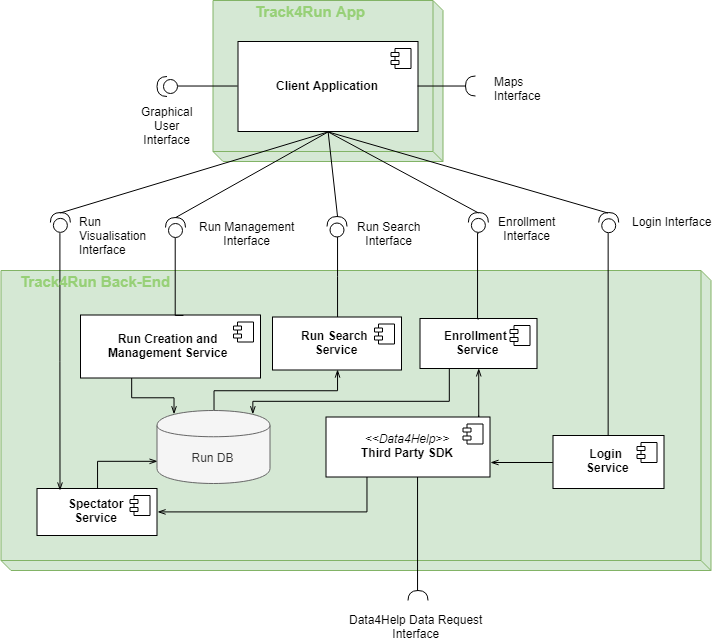
\includegraphics[width=\columnwidth]{ComponentDiagrams-Track4Run.png}
	\caption{Track4Run Components}
\end{figure}
\FloatBarrier



\subsection{Deployment View}

\FloatBarrier
\begin{figure}[!h]
	\centering
	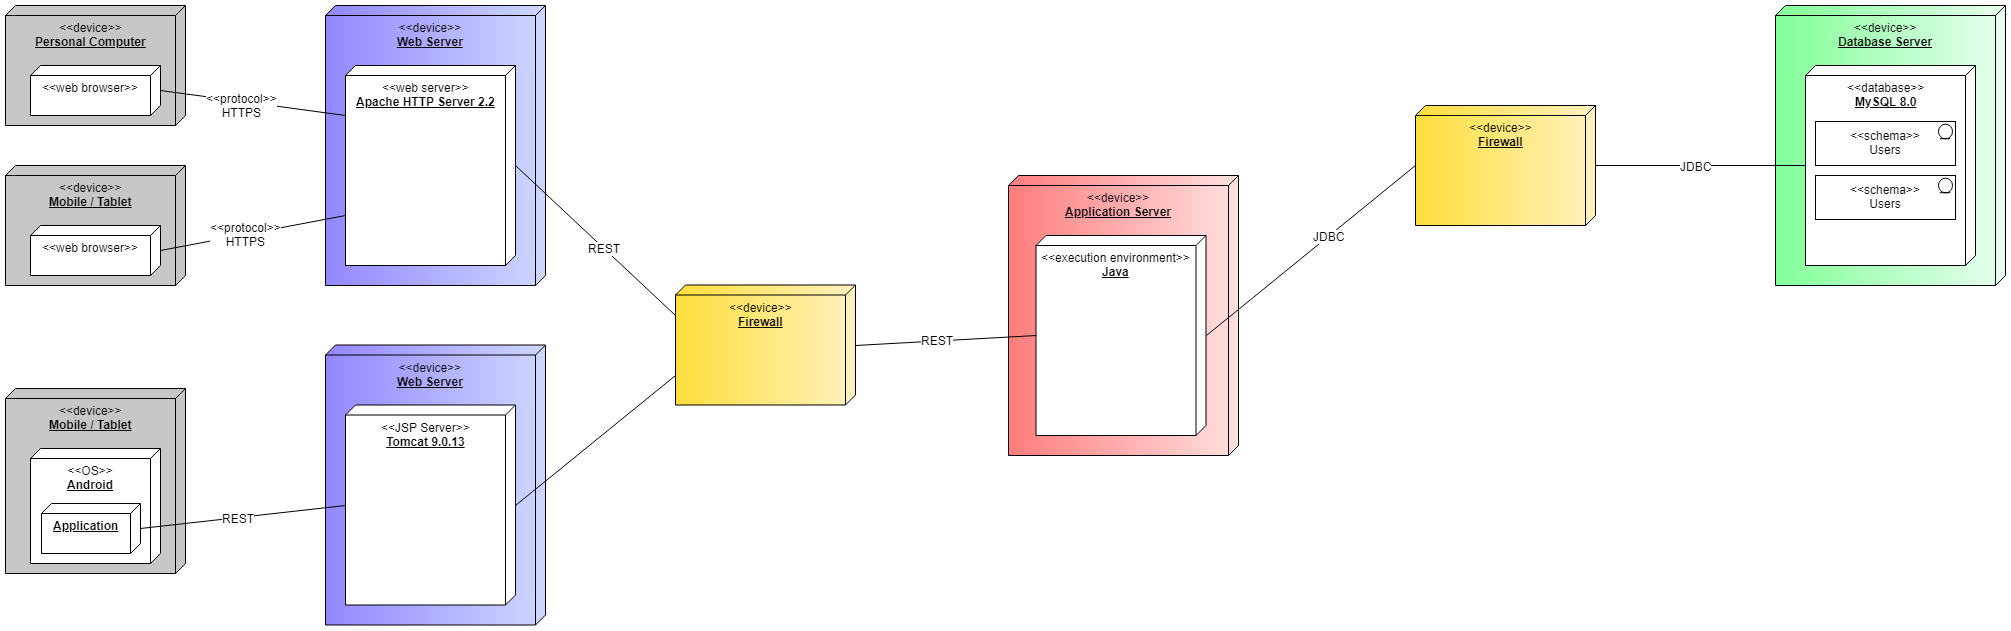
\includegraphics[angle=90, height=0.9\textheight]{deploymentDiagram.png}
	\caption{Track4Run Components}
\end{figure}
\FloatBarrier

\subsection{Runtime View}
- Auth
- One-shot req
- Subscription req
- New data arrives

\subsection{Component Interfaces}
\subsection{Selected Architectural Styles and Patterns}
- stateless
- microservice
- monolithic
- token auth
- loose coupling
- event driven and message queues
- server side service discovery
\subsection{Other Design Decisions}
- NOSQL DB
- JWT
- REST
- RabbitMQ